\subsection{The Large Hadron Collider}
\begin{frame}{The Large Hadron Collider (LHC)}
\begin{columns}
\column{0.4\textwidth}

\begin{itemize}
    \item \textbf{\textcolor{structurColor}{$pp$ collisions,} up-to 13 TeV}
    \item Collision rate of $\sim$ 40 MHz (\textbf{\textcolor{HHred}{challenging trigger}})
    \item\textbf{ Four large experiments} 
\end{itemize}
\column{0.6\textwidth}
\begin{figure}
        \centering
        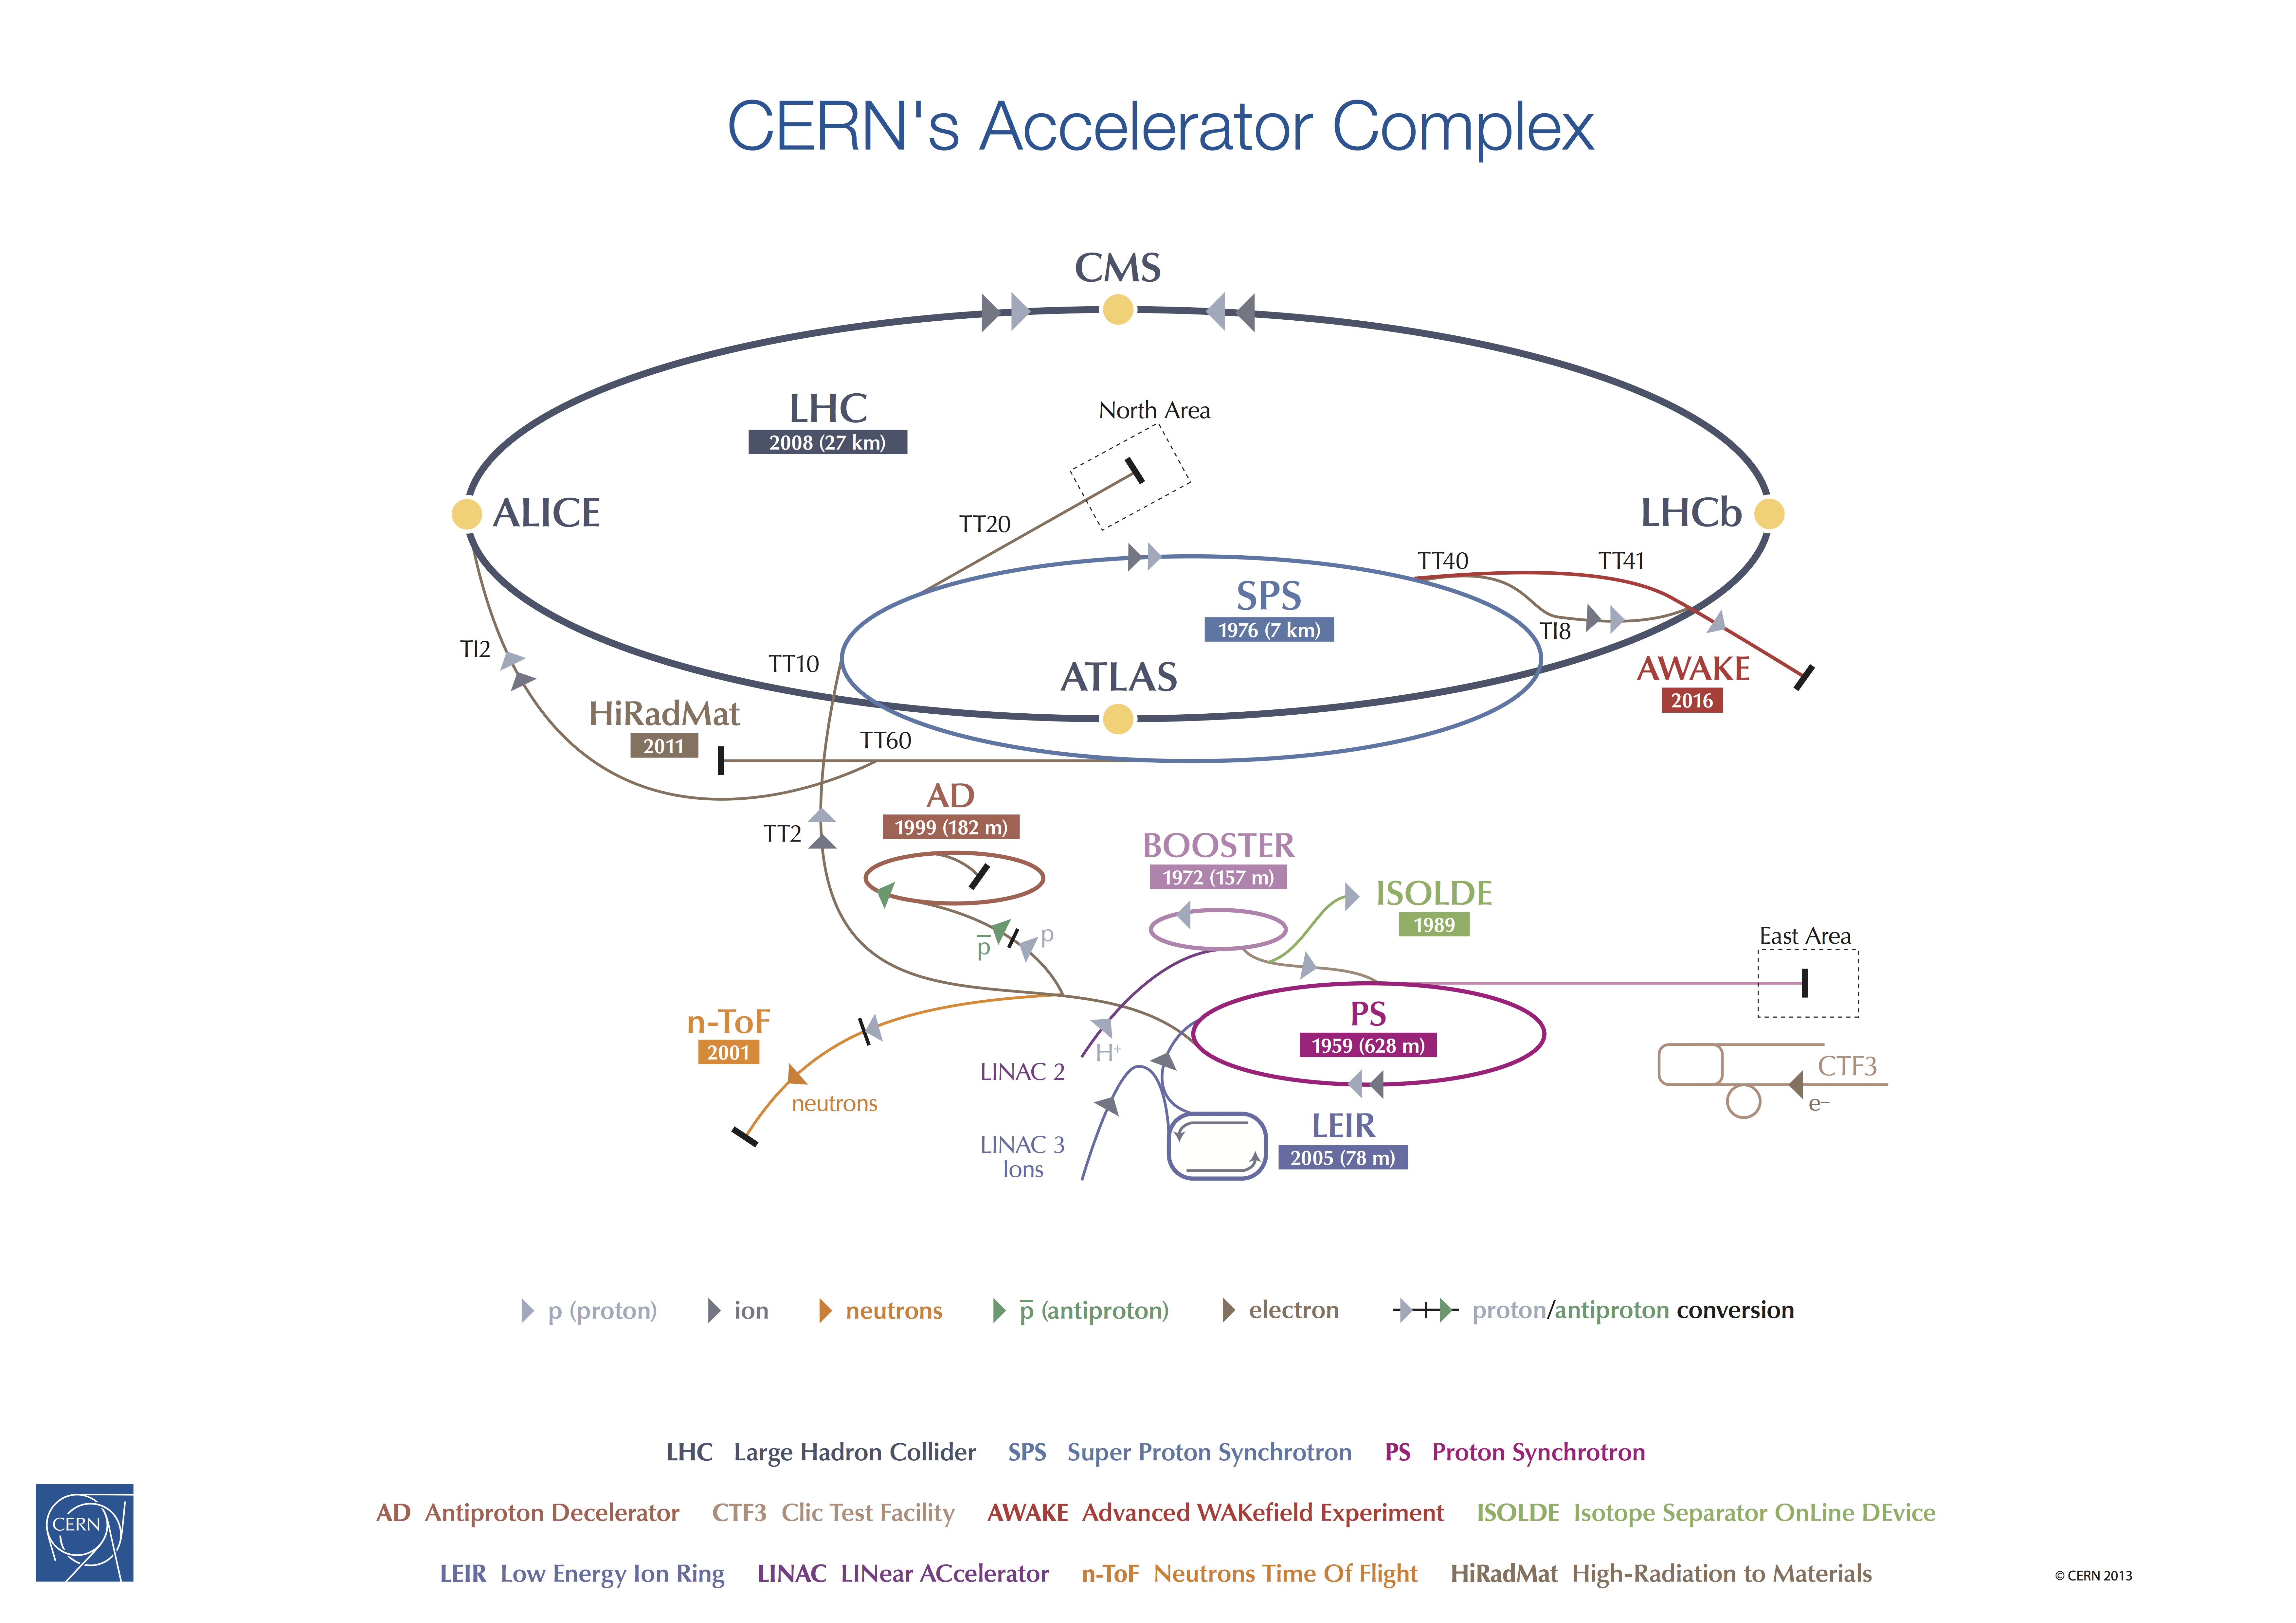
\includegraphics[width=1.1\textwidth]{Part2/Img/LHC_chain.jpeg}
\end{figure}    
\end{columns}

\end{frame}

\subsection{The ATLAS detector}
\begin{frame}{The ATLAS detector}

\begin{columns}
\column{0.7\textwidth}
\begin{figure}
    \centering
    \includegraphics[width=1.\textwidth]{Part2/Img/ATLAS_sketch.jpg}
\end{figure}

\column{0.3\textwidth}

\begin{itemize}
    \item \textbf{different sub-detecto}r 
    \item \textbf{cylindrical} coordinate system
\end{itemize}
\begin{equation*}
    \textcolor{HHblue}{\eta = -\ln[\tan\frac{\theta}{2}]}
\end{equation*}
\begin{figure}
    \centering
    \includegraphics[width=1.\textwidth]{Part2/Img/ATLAS_Sys.jpeg}
\end{figure}

\end{columns}

\end{frame}

\subsection{Particles reconstruction}
\begin{frame}{Particles reconstruction}

\begin{columns}
\column{0.4\textwidth}

\begin{itemize}
    \item \textcolor{HHred}{Electrons} \& \textcolor{HHred}{Photons}
    \begin{itemize}
        \item EM cluster (+ ID track)
    \end{itemize}
    \item \textcolor{cadmiumorange}{Muons}
    \begin{itemize}
        \item Tracks
    \end{itemize}
    \item \textcolor{applegreen}{Hadrons} (jets)
    \begin{itemize}
        \item EM/Had clusters (+ ID track)
    \end{itemize}
    \item \textcolor{HHturquoise_l}{Neutrinos}
    \begin{itemize}
        \item Missing momentum
    \end{itemize}
\end{itemize}
\column{0.6\textwidth}
\begin{figure}
    \centering
    \includegraphics[width=1.\textwidth]{Part2/Img/Particle_detection.jpg}
   
\end{figure}

\end{columns}

\end{frame}

\subsection{Luminosity and Pile-up}
\begin{frame}{Run 2 data taking}
    
\begin{columns}
\column{0.4\textwidth}
\textcolor{HHred}{\underline{Luminosity}}:
\begin{itemize}
    \item Data-taking efficiency $>$ 90\%
    \item Integrated luminosity \\ $\mathcal{L}_{int}$ = 139 fb$^{-1}$
\end{itemize}
\textcolor{HHblue}{\underline{Pile-up}}:
\begin{itemize}
    \item Dense environments 
    \item \textbf{challenge!}
\end{itemize}

\begin{figure}
    \centering
     \fcolorbox{HHblue}{HHwhite2}{
    \includegraphics[width=0.8\textwidth]{Part2/Img/PileupEvent.png}
    }
\end{figure}
\column{0.6\textwidth}

\begin{figure}
    \centering
     \fcolorbox{HHred}{HHwhite2}{
    \includegraphics[width=0.55\textwidth]{Part2/Img/intlumivstimeRun2DQall.pdf}
    }
\end{figure}

\begin{figure}
    \centering
     \fcolorbox{HHblue}{HHwhite2}{
    \includegraphics[width=0.55\textwidth]{Part2/Img/mu_2015_2018.pdf}
    }
\end{figure}

\end{columns}  
\end{frame}

\begin{frame}{Upgrade plans: Run-3 and HL-LHC}
    \begin{figure}
        \centering
        \includegraphics[width=0.6\textwidth]{Part2/Img/HL-LHC-plan-2021-1.pdf}
    \end{figure}
\begin{columns}
\column{0.5\textwidth}  
\begin{center}
    Run-3
\end{center}
\begin{itemize}
    \item $\sqrt{s}=$ 13.6 TeV
    \item $\mathcal{L}_{int}$ = 350 fb$^{-1}$
\end{itemize}
\column{0.5\textwidth}  

\begin{center}
    HL-LHC
\end{center}
\begin{itemize}
    \item $\sqrt{s}=$ 14 TeV
    \item $\mathcal{L}_{int}$ = 3000 fb$^{-1}$
\end{itemize}

\end{columns}
\end{frame}

{
\usebackgroundtemplate{\includegraphics[width=1.03\paperwidth]{Img/figaux_01}}
\begin{frame}
\end{frame}
}


\begin{frame}{Where are we?}
\begin{columns}
\column{0.4\textwidth}    

\begin{figure}
    \centering
    \fcolorbox{applegreen}{HHwhite2}{
    \includegraphics[width=0.8\textwidth]{Part2/Img/36ifb_limit.pdf}
    }
\end{figure}

\column{0.6\textwidth}    
\begin{itemize}
    \item \textbf{\textcolor{applegreen}{2015-2016 data (36$^{-1}$)}}
    \begin{itemize}
        \item $\frac{\sigma_{HH}}{\sigma_{HH}^{SM}}$ limit: \textbf{\textcolor{structurColor}{22}} (Exp. \textbf{28})
        \item $\kappa_{\lambda}$ constrain: \textbf{\textcolor{structurColor}{[-8.2, 13.2]}} (Exp. \textbf{[-8.3, 13.2]})
    \end{itemize}
\pause    
    \item \textbf{\textcolor{HHred}{Full run-2 data (139$^{-1}$)}}
\end{itemize}    
\begin{tabular}{lcccc}
    \hline 
    \hline
    & Single H & HH & HH$\to b\bar{b}\gamma\gamma$ & $\sim$10\% eff. \\
     \hline
    Events &  6.7M  & 4.3k & 13 & 0-1 \\
      \hline\hline 
\end{tabular}    
\end{columns}
\end{frame}